\documentclass[11pt]{article}
\textheight 9in
\textwidth 6.5in
\oddsidemargin 0in
\topmargin 0in
\headheight 1in
\headsep 0in
\usepackage{color}
\usepackage{lastpage}
\usepackage{graphicx}
\usepackage{fancyhdr}
\pagestyle{fancy}
\cfoot{}
\rhead{\thepage\ of \pageref{LastPage}}
% \renewcommand{\headrulewidth}{0pt}
\usepackage[top = 4em, headsep=.2in]{geometry}
\usepackage{textcomp}
\usepackage{enumitem}

\usepackage{bm}
\begin{document}

\noindent{{\textbf{\large Spring 2020  \hfill Stat 305 (Section 4)
\hfill %Page \thepage   { of }  \pageref{lastpage}
Final}}

\vspace{2em}

\noindent\framebox(200, 50){\vspace{3em}\hspace{2em}\bf Name: \hspace{6cm}}

\bigskip

\noindent\emph{Total points for the exam is 100. Points for
individual questions are given at the beginning of each problem.
Show all your calculations clearly. Put final answers in the box at
the right (except for the diagrams!).}


\bigskip


%
\noindent {\bf 1.}\hfill[2+2+4+5+4+5+4+4+6=36 points] \\
%
\noindent The data used in creating the 
regression analysis JMP output on page 13-14 come from a metal-cutting drilling experiment. The explanatory variables studied were\\

$x_1$ = natural logarithm of the diameter of the drills 

$x_2$ = natural logarithm of the feed rate (rate of drill penetration into the workpiece) of the drills\\

\noindent and the response variable was\\

$y$ = natural logarithm of the thrust required to rotate the drill on an aluminum alloy\\

\noindent Use the {\bf first} regression analysis output in
answering the questions (a)-(d) below.

\begin{enumerate}



\item[(a)] What fraction of the observed raw variation in
$y$ is explained using $x_1$ as a predictor variable?

\hfill \hfill\framebox(150, 30)[l]{\, fraction = }

%\hfill \fbox{ \textcolor[rgb]{1.00,1.00,1.00}{$\bigcap$} \hskip
%-0.4cm (ii) probability= \hspace{1.9cm}}

%\hfill \fbox{ \textcolor[rgb]{1.00,1.00,1.00}{$\bigcap$} \hskip
%-0.4cm For equation 2:\hspace{3cm}}

\vskip 4cm

\item[(b)] What is the sample correlation between $y$ and $\hat y$?
 (Give a number.)


\hfill \hfill\framebox(150, 30)[l]{\, corr= }

\vskip 3cm

\newpage
\item[(c)] Give a 95\% two-sided confidence interval for the
\emph{increase} in mean value of natural logrithm of thrust ($y$) associated with a 0.5 unit
increase in natural logrithm of the drill diameter ($x_1$). (No need to simplify.)



%\vskip 1.5cm

 \hfill\framebox(300, 30)[l]{\, conf. interval = }

 \vskip 8cm



\item[(d)] As it turns out, the data have $\bar x_1= -1.145$
 and $\sum (x_{1i} - \bar x_1)^2 = 0.475$. Use these facts
and give a 90\% lower confidence bound for the mean natural logarithm of thrust ($y$) when
natural logarithm of drill diameter  equals $-1$ (i.e. $x_1 = -1$). (No need to simplify.)



%\vskip 1.0cm

 \hfill \framebox(300, 30)[l]{\, lower conf. bd = }


\end{enumerate}
\newpage
\noindent Use the {\bf second} regression analysis
output in answering the questions (e)-(i) below. The standard error of the predicted mean response $\hat{\mu}_{y|\bm x}$ for the second regression analysis is in the last column of the data table.\\

\begin{enumerate}
\item[(e)] Give the residual corresponding to the second
observation ($x_1= -0.901,x_2 = -5.116$, and $y = 5.927$).



 \hfill \framebox(200, 30)[l]{\, residual = }
\vskip 4cm
\item[(f)] Give a 90\% upper prediction bound for the next natural logarithm of thrust ($y$) when $x_1 = -0.901$ and $x_2 =-5.116$. (No need to simplify.)

% \vskip 1.5cm

%\vskip 1.0cm

 \hfill \framebox(300, 30)[l]{\, upper pred. bd = }
\vskip 7cm

\item[(g)] Find the value of a $t$-statistic, its degrees of
freedom, and the corresponding $p$-value for testing whether the
predictor $x_2$ can be dropped from this multiple linear regression
model. What is your conclusion? (\emph{Hint: If the slope is zero, the predictor is of no use to predict the response and therefore can be dropped.})


\framebox(120, 30)[l]{\, 
 Observed $t =$ }
 %
 \hfill
 %
\framebox(120,30)[l]{\, df =}
 %
 \hfill
\framebox(120,30)[l]{\, 
 $p$-value = }\\
 %
Conclusion (circle only one): \hfill 

\hskip 2cm(a) $x_2$ should be dropped
% \hfill 

\hskip 2cm(b) $x_2$ should not be dropped


\item[(h)] Give  the value of an $F$ statistic, its degrees of freedom, and the
corresponding $p$-value for testing $H_0: \; \beta_1=\beta_2=0$
against $H_a:\; $ not $H_0$. What is your conclusion?

\vskip 0.25cm

\framebox(120, 30)[l]{\, 
 Observed $F =$ }
 %
 \hfill
 %
\framebox(60,30)[l]{\, df\textsubscript{1} =}
 %
 \hfill
 \framebox(60,30)[l]{\, df\textsubscript{2} =}
 %
 \hfill
\framebox(120,30)[l]{\, 
 $p$-value = }\\
 %

Conclusion (circle only one):

\hskip 2cm(a) $x_1, \; x_2$ should be
dropped 

\hskip 2cm(b) $x_1, \; x_2$ should not be dropped

\item[(i)]Fitting the complete second-order model
%
$$y = \beta_0 + \beta_1 x_1+ \beta_2 x_2+ \beta_3 (x_1)^2+ \beta_4
(x_2)^2 + \beta_5 (x_1 x_2) + \epsilon$$
%
gave $SSR$ = 1.1093 and $SSE=0.01715$. Find the value of an $F$
statistic and its degrees of freedom for testing whether all the
second order predictors  (i.e.  $(x_1)^2, (x_2)^2$ and $(x_1 x_2)$)
can be dropped from the complete second-order model involving all 5
predictors. What is your conclusion.?

\vskip 8cm

\framebox(120, 30)[l]{\, 
 Observed $F =$ }
 %
 \hfill
 %
\framebox(60,30)[l]{\, df\textsubscript{1} =}
 %
 \hfill
 \framebox(60,30)[l]{\, df\textsubscript{2} =}
 %
 \hfill
\framebox(120,30)[l]{\, 
 $p$-value = }\\
 %

Conclusion (circle only one):

\hskip 2cm(a) $(x_1)^2, (x_2)^2, (x_1 x_2)$ should be dropped

\hskip 2cm(b) $(x_1)^2, (x_2)^2, (x_1 x_2)$ should not be dropped

\end{enumerate}

\newpage
\noindent {\bf 2.}\hfill[3+6+4=13 points] \\
%
 Two independent discrete random variables $X$ and  $Y$
 can be described using the following probability functions:

\begin{table}[ht]
\begin{minipage}[b]{0.5\linewidth}\centering
\begin{tabular}{c|cccc}
%\hline
$x$ &$-2$& 0&1&5\\
\hline
$f_X(x)$ & 0.1&0.4 & 0.2&0.3\\
%\hline
\end{tabular}
\end{minipage}
\hspace{0.5cm}
\begin{minipage}[b]{0.5\linewidth}
\centering
\begin{tabular}{c|cccc}
%\hline
$y$ &0& 1&2&3\\
\hline
$f_Y(y)$ & 0.2&0.4 & 0.3&0.1\\
%\hline
\end{tabular}
\end{minipage}
\end{table}
%

\begin{enumerate}

\item[(a)] Find the cumulative probability function for $X$.

\vskip 5cm

\item[(b)] Find the means and standard deviations for $X$ and $Y$
respectively.


 \hfill
\framebox(200, 30)[l]{ \,
$\mu_X$ = \hspace{2cm} $\sigma_X=$\hspace{2cm}}

 \hfill
\framebox(200,30)[l]{ \,
$\mu_Y$ = \hspace{2cm} $\sigma_Y=$\hspace{2cm}}


\vskip 8cm

\newpage
\item[(c)] Find  the mean and standard deviation
for the random variable $3X - 5Y + 2$.



 \hfill
\framebox(200, 30)[l]{\, mean
= \hspace{2cm} s.d=\hspace{2cm}}

\end{enumerate}

\newpage

\noindent {\bf 3.}\hfill[4+4+3+6+5=22 points] \\
%
 The spring constants of two types of steel springs are measured. The resulting measurements and some summary statistics are given below.

\begin{center}
\begin{tabular}{|p{3cm}|p{3cm}|}
\hline
Type 1 Springs  & Type 2 Springs\\
\hline
1.99, 2.06, 1.99, 1.94, 2.05, 1.88, 2.30   & 2.85, 2.74, 2.74, 2.63, 2.74, 2.80\\
$\bar{x}_1 = 2.03$ & $\bar{x}_2 = 2.75$\\
$s_1 = 0.134$ & $s_2 = 0.074$\\
\hline
\end{tabular}
\end{center}

\begin{enumerate}

\item[(a)]  Give a 95\% upper prediction bound for the
spring contant of the next Type 1 spring. (No need to simplify.)



 \hfill \framebox(400, 30)[l]{\, upper pred. bd (Type 1)= \hspace{6cm} }
\vskip 7cm
\item[(b)] Give a a 95\% lower confidence bound for the
mean spring contant for Type 1 springs. (No need to simplify.)

%\vskip 1.0cm

 \hfill \framebox(400, 30)[l]{\, lower conf. bd (Type 1)= \hspace{6cm} }
 \vskip 7cm

\item[(c)] What assumptions have to be made in order to construct the
confidence bound in part (b)?

\vskip 3cm

\item[(d)]  Give a 95\% two sided confidence interval for the
difference in mean spring constants for the two types of springs.
(No need to simplify.)

% \vskip cm

%\vskip 1.5cm

 \hfill \framebox(400, 30)[l]{\, conf. interval = }

\vskip 10cm
\item[(e)] What assumptions have to be made in order to construct the
confidence interval in part (d)?

\vskip 1.cm

\end{enumerate}


\newpage

\noindent {\bf 4.}\hfill[5+5+5=15 points] \\
%
Jars of a particular type are made in a factory. The jars have weights with mean 120 g and standard deviation 1.6 g.
%
\begin{enumerate}
%
\item[(a)] Assume that the weights are normally distributed 
 and specifications on the
weights are 120 g $\pm$ 4 g.  What  fraction of the weights of jars actually satisfy this specification ?

%What does $\mu$ need to be in order to achieve this fraction?

 \hfill
\framebox(150, 30)[l]{\, 
fraction = \hspace{3cm}}
\vskip 6cm


\item[(b)] Evaluate the probability that \emph{at most} 11 of the next 12 jars produced are within the
specifications of 120 g $\pm $ 4 g.

 \hfill
\framebox(150, 30)[l]{\, probability = \hspace{3cm}}

\newpage
\item[(c)] Let $\bar X$ denote the sample mean weight of 80 jars
of this type. Approximate the probability that $\bar X$ is bigger than 120.1 g.



 \hfill
\framebox(150, 30)[l]{\, probability = \hspace{3cm}}

\end{enumerate}

\newpage

\noindent {\bf 5.}\hfill[7+7=14 points] \\
%
An experiment was made in order to measure the compressive strength of 6 different concrete formulas. The data, some summary statistics, and the
analysis of variance table are given below.
%
\begin{center}
\begin{tabular}{|c|c|c|}
\hline
Formula 1  & Formula 2 & Formula 3 \\
\hline
5659, 6225, 5376 & 5093, 4386, 4103 & 3395, 3820, 3112 \\
$\bar{y}_1 = 5753.33$ & $\bar{y}_2 = 4527.33$& $\bar{y}_3 = 3442.33$\\
$s_1 = 432.29$ & $s_2 = 509.91$ & $s_3 = 356.37$\\
\hline
 Formula 4 & Formula 5 & Formula 6\\ \hline
2971, 3678, 3325 & 2122, 1372, 1160 & 2051 , 2631 , 2490  \\
$\bar{y}_4 = 3324.67$ & $\bar{y}_5 = 1551.33$ & $\bar{y}_6 = 2390.67$\\
$s_4 = 353.50$ & $s_5 = 505.45$ & $s_6 = 302.49$ \\ \hline

\end{tabular}
\vskip 1cm ANOVA Table\\
\vskip 0.2cm
\begin{tabular}{|l|r|r|r|r|}
\hline
Source & DF & Sum of Squares & Mean Square & F-ratio\\
\hline
Model  & 5 & 33584690 & 6716938 & 38.5359 \\
%\hline
Error   & 12  & 2091642  & 174304  & (Prob $>$ F) $<$ 0.0001\\
\hline
Total    & 17 & 35676332 & &    \\
\hline
\end{tabular}
\end{center}

Let $\mu_1, \mu_2, \mu_3, \mu_4, \mu_5$ and $\mu_6$ be the true compressive strength
for concrete formula 1 to formula 6.

\begin{enumerate}
%
\item[(a)] Give a 95\% two-sided confidence interval
for the quantity $\frac{1}{2}(\mu_2 + \mu_3) - \mu_4$. (No need to
simplify).

 \hfill \framebox(400, 30)[l]{\, conf. interval = }
\vskip 8cm

%\vskip 1.5cm


\newpage
\item[(b)] Assess the strength of the evidence
against $H_0: \mu_1=\mu_2=\mu_3=\mu_4 = \mu_5 = \mu_6$ in favor of $H_a:$ not $H_0$.
(Show all steps!)

\end{enumerate}
\newpage


\clearpage

\centering

\section*{JMP Output}

\subsection*{Data Table}
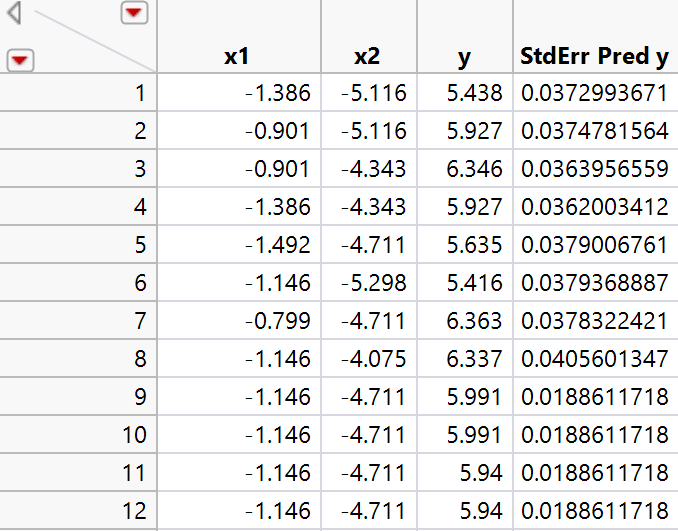
\includegraphics[width = 0.6\textwidth]{./table.PNG}

\subsection*{Regression 1}

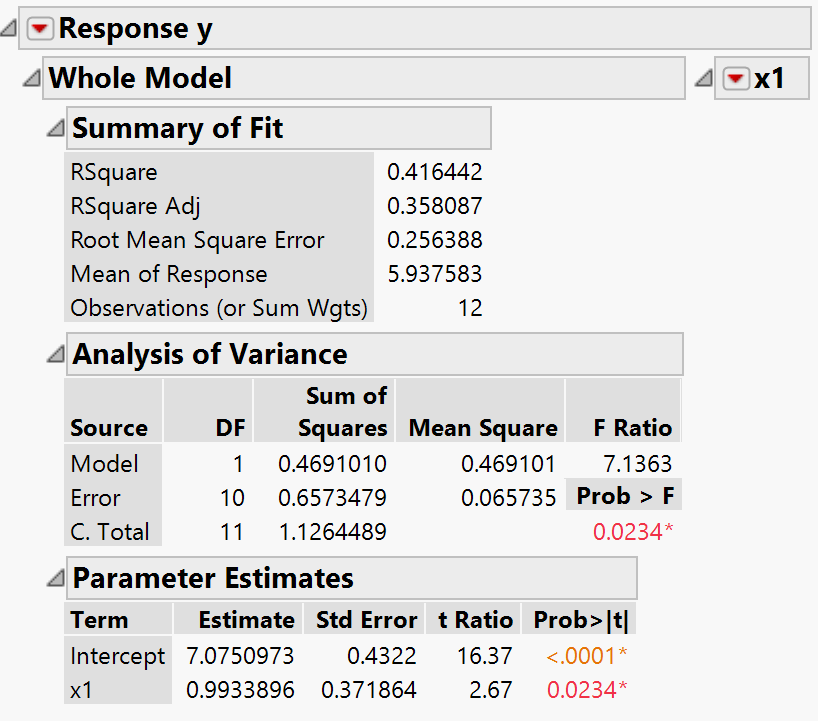
\includegraphics[width = 0.6\textwidth]{./model1.PNG}

\subsection*{Regression 2}
\centering
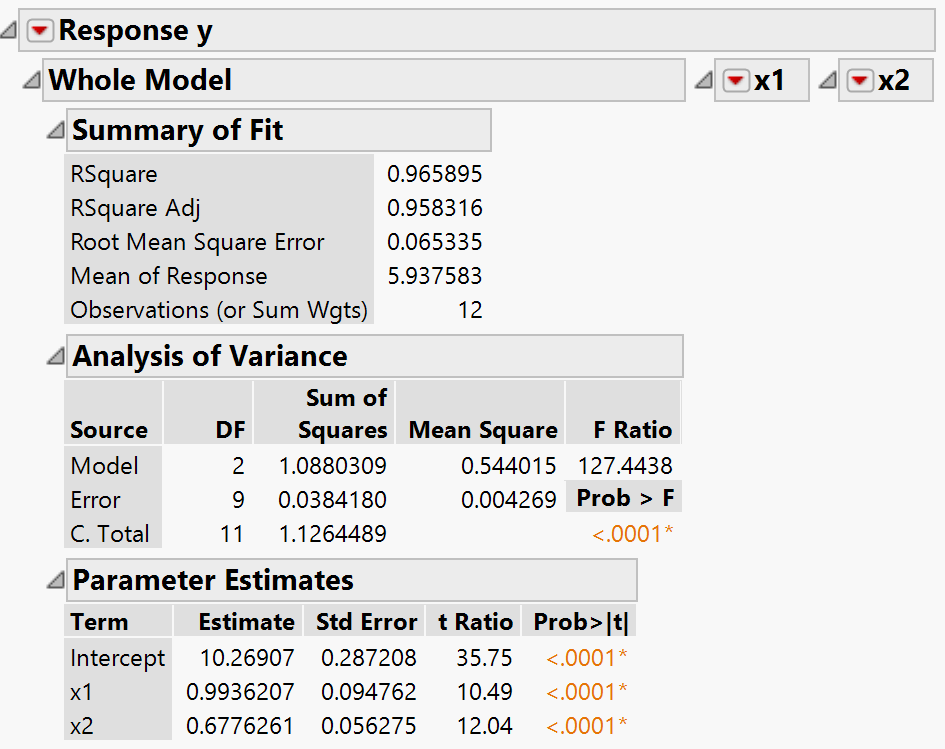
\includegraphics[width =0.6\textwidth]{./model2.PNG}
%
\label{lastpage}


\end{document}
